
\chapter{Instrumentation}

\label{Chapter4}


\large{


\section*{Introduction}


A four-dish interferometer was built at the Mauritius Radio Telescope observatory site Bra D'EAU in the Flacq district to study the HI emission line and serves as a prototype instrument for the SKA outstation Mauritius. This is where the renowned Mauritius Radio Telescope MRT is located. It was built to complement the Cambridge 6C survey, a radio map of the northern sky at 150MHz \cite{somanah2013astrophysical}. The system is being set up as the Mauritius first parabolic dish reflector antenna interferometer, suitable for a range of radio astronomy experiments and the development of technical expertise for SKA project.

The content of the three chapters dealing with the experimental component of this thesis is as follows:
Chapter 6 Instrumentation. Development and performance verification of the Mauritius Small Dish Array (MSDA) system are described in figure \ref{fig:4.1}.

Chapter 7 Measurement Results. Measurements to evaluate the performance of the MSDA itself—gain, noise performance and radiation patterns ..............edit.
Chapter 8 Discussion of Results. Discussion of the MSDA evaluation measurements. The results are compared with predictions based on the dish structure and the MSDA .................edit.

\begin{figure}[h!]
    \centering
\includegraphics[width=6in]{Figures/MSDA1.jpg}
\caption{The four-dish prototype radio telescope is located at MRT; the west antenna is antenna-four (A4) in the foreground, antenna-three (A3), antenna-two (A2) in the background, and the far-eastern antenna-one (A1) with the feed horn mounted on top.}
 \label{fig:4.1}
\end{figure}




%The complete system involves the reflector, feed, low noise amplifiers, noise calibration system, frequency converters, digital spectrometers, continuum signal processing, and monitor and control system. The
%main parameters of this front-end are the antenna efficiency
%\(\eta\) and the system noise temperature, Tsys. Our goal is an \(\eta\)
%of \(\ > \) 40 \% from 1.2 to 14 GHz with typical values of 55\%,
%and a maximum Tsys of 55K over the band with 35K at best
%frequencies. These values of Tsys include 2.7K cosmic
%background, .3K of atmosphere, and .5K allocated for
%spillover and feed support reflections of ground radiation so
%10K must be added the noise temperature of feed and LNA


\section{Overview}
The MSDA Interferometer was built during 2005 and 2006 with improvements
to the system, mainly in the operating software and beamformer firmware,
continuing during the life of the instrument. In January 2009 there was
a major equipment failure in the system.This failure was not repaired as
CSIRO’s FPA technology development focus had moved to a new test bed
built adjacent to the Parkes 64 m radiotelescope and sufficient data had been
gathered on the NTD Interferometer.
The primary specifications for the MSDA instrument are shown in Table
\ref{tab:4.1}. A block diagram of the system is shown in Figure \ref{fig:4.1} and a more detailed signal flow diagram in Figure \ref{fig:4.2}.
The system was developed by project two research students.
 The author took prime responsibility of developing the array, the mechanical structures,control and monitoring and the feed system. Although basic beamforming was demonstrated at this time, a methodical approach to understanding, optimizing and stabilizing the system was undertaken by the author. This provided more consistent results and facilitated demonstrating
the maximum G/T beamforming weighting. The following list clarifies the
attributions for the NTD Interferometer project:
6.3 Reflectors. This work was performed by Mike Kesteven, external con


\begin{figure}
    \centering
\includegraphics[width=6in]{Figures/SCHEMATIC-DIAGRAM-DASPA.png}
\caption{Concrete column Pad footing foundation with the design parameters}
 \label{fig:4.1}
\end{figure}






\begin{table}[h!]
    \centering
\caption{\textbf{MSDA Interferometer specification}}
\begin{tabular}{ c   c}
    \hline
 Dish Diameter & 2.4m  \\ 
 Dish F/D & 0.65  \\  
 Frequency range & 1 - 2GHz \\
 Instantaneous bandwidth & 100MHz \\
 Mount system & Azimuth / Elevation\\
 Number of antenna separations & 6\\
 Feed type & Offset feed \\
 \hline
 \end{tabular}
    \label{tab:4.1}
\end{table}




6.4 The array design and configuration. This section is the author’s work including of the designing and installations of the antenna control  system.

6.5 Feed system. The design of the feed system was the author’s.  The higher level software control and calibration method was the author’s work.
6.6 Receiver. The SNAP board receivers were designed by Mr Paul Akumu.


6.8 Instrument Control and Data Collection. The basic system control functionality including the data processing was augmented by the author as
described in this section.

6.9 System Level Commissioning Tests. This was the author’s work.

6.10 Element Gain Stability. This was the author’s work.

6.11 Radio Sources. Suitable radio sources for this work were identified by
,,,,,,, and the author




\subsection{REFLECTOR}
The four 2.4m parabolic reflectors were a donation from the Mauritius telecommunications company as redundant offset satellite dishes and were later refurbished for use as radio astronomy antennas. The parabola has a solid surface made of fiberglass material. Originally, the dishes were designed to be used as geostationary antennae. To accommodate a tracking system with new motor, encoder, and control system designs, the reflector bracket had to be rebuilt. The mechanical design of the antenna and the material selections were built to accommodate the local climatic conditions at the MRT site, which is roughly 3 kilo-meters from the ocean.
The reflectors are symmetrical parabolas with a 2.4 m diameter shown and a 0.65 focal length to diameter ratio. The azimuth and elevation mounts make it easier to track celestial radio sources. Figure \ref{fig:4.2} shown the symmetrical parabolas being assemble.
Section 5 addresses this. . %Sky coverage is however limited to ±3h44’ (±56°) in hour angle and -83°, +16° in declination

\begin{figure}
    \centering
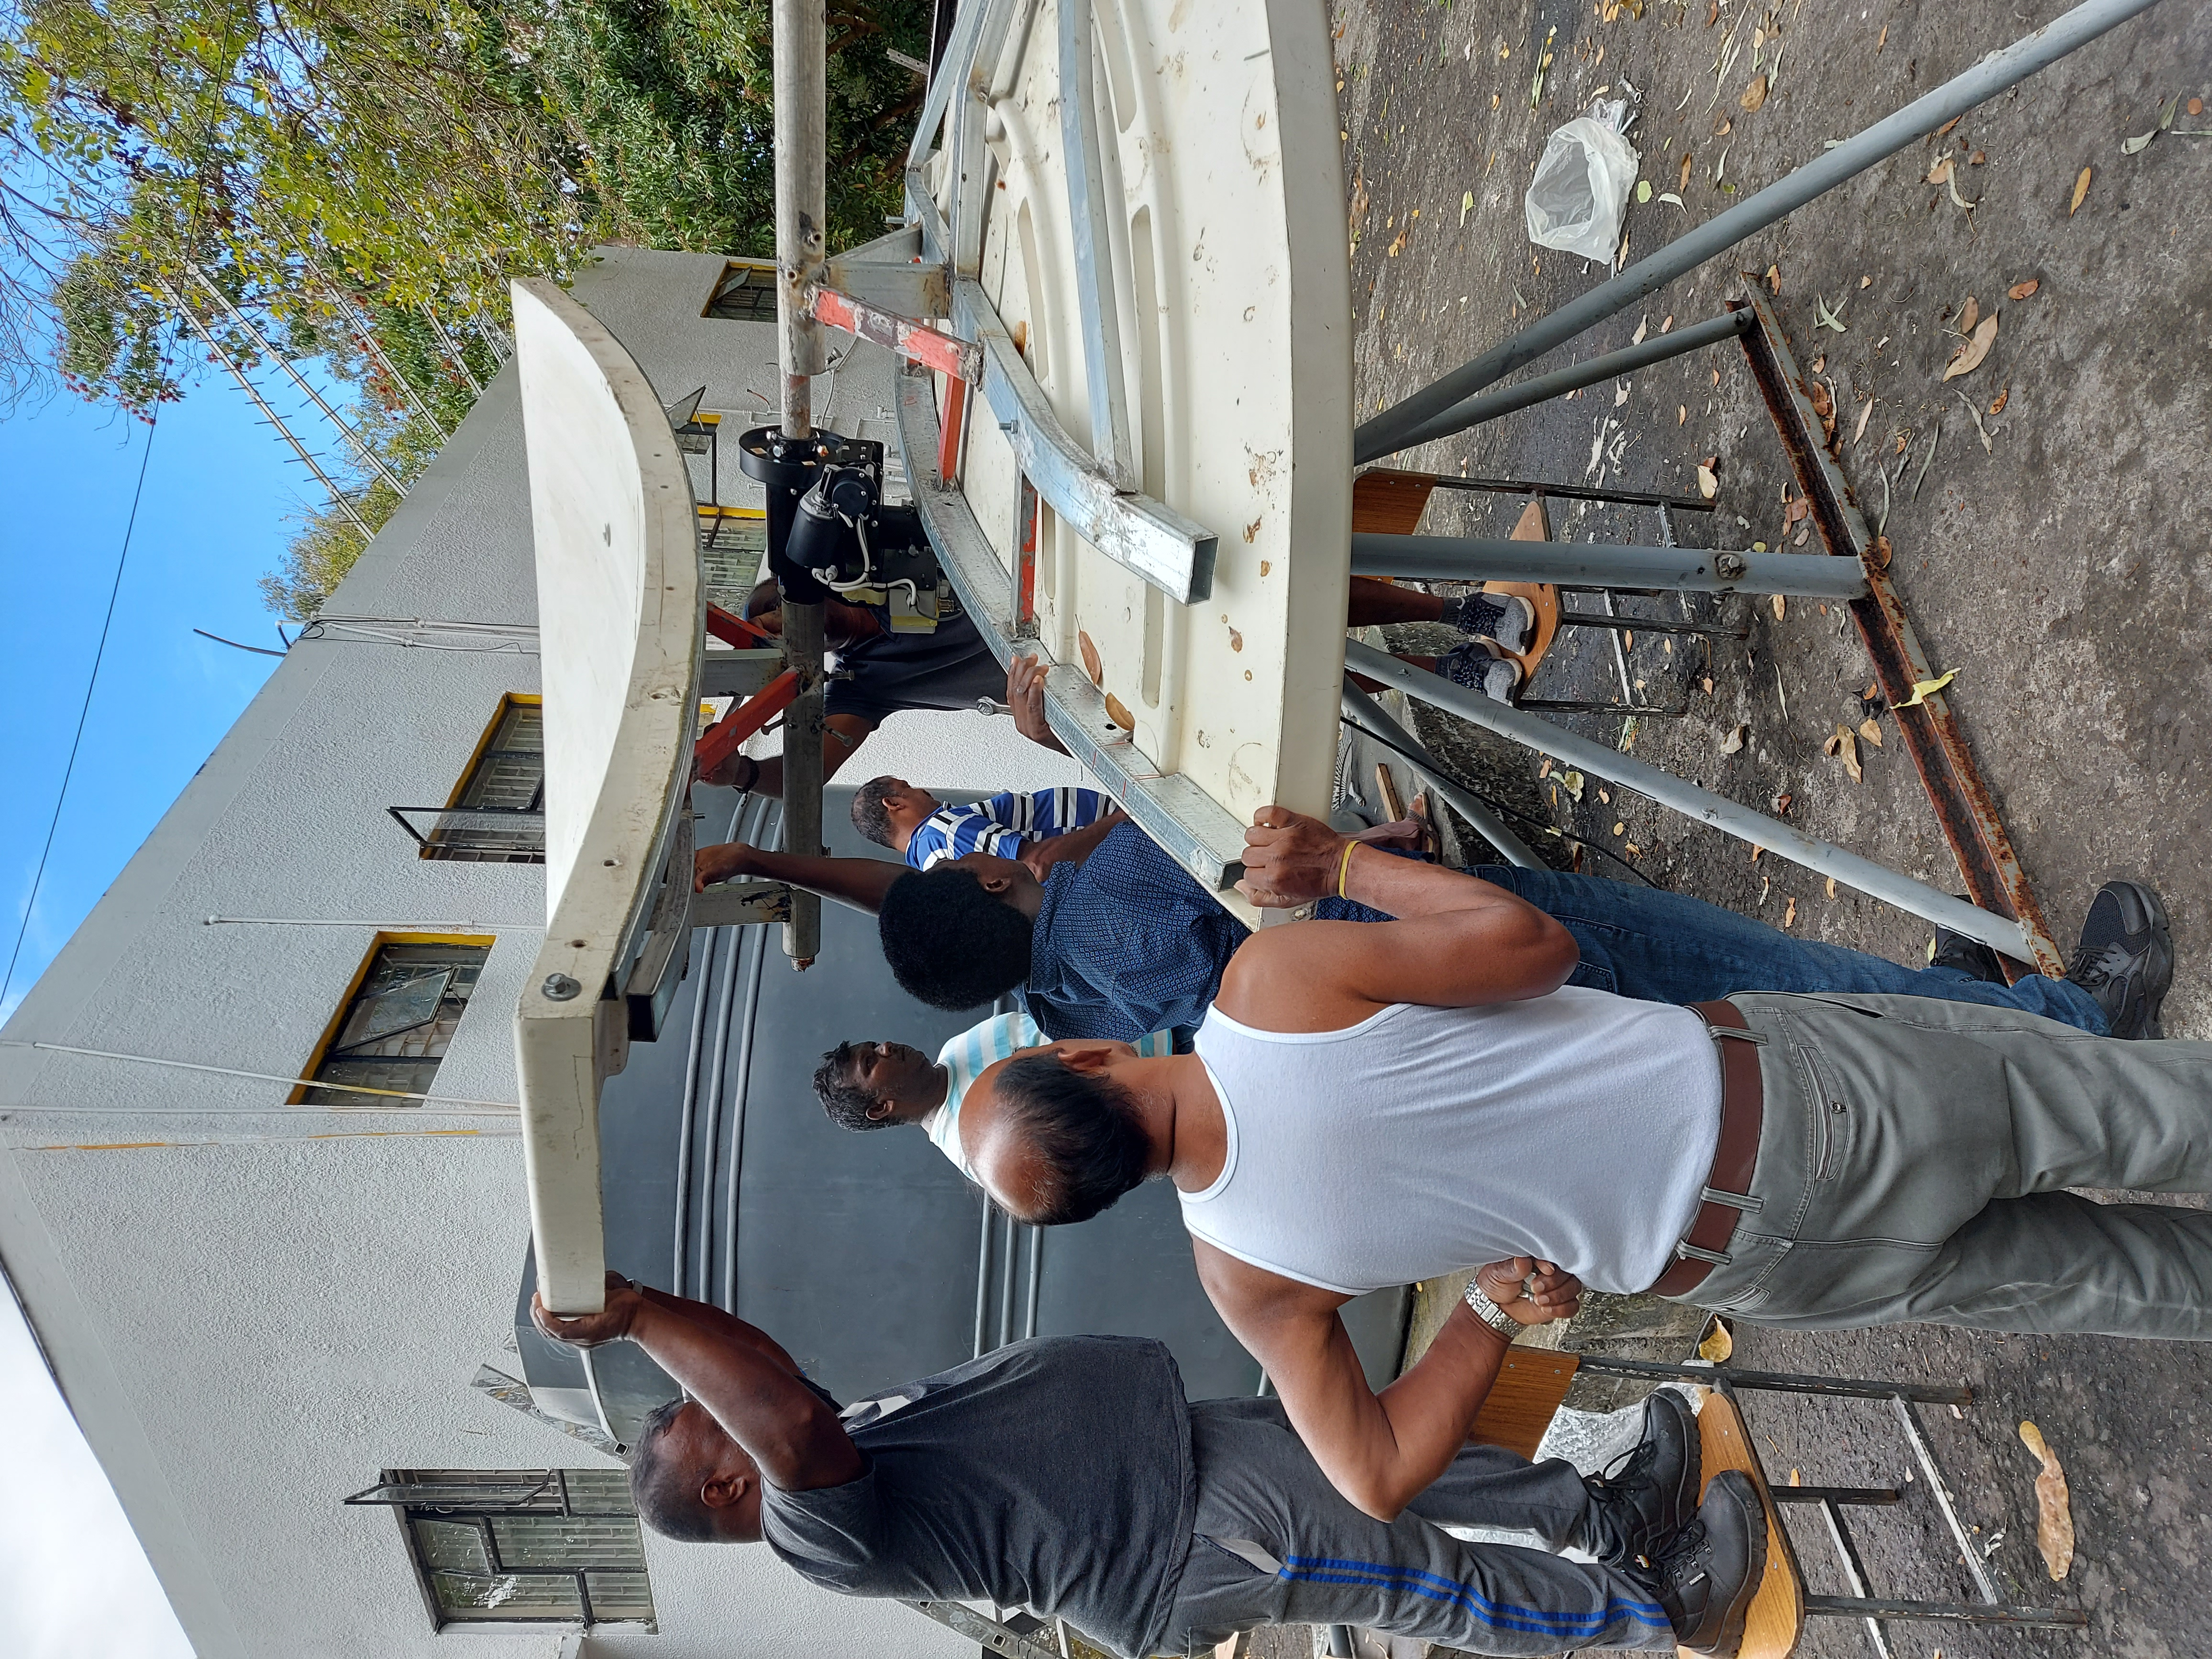
\includegraphics[width=6in]{Figures/telesscope construction.jpg}
\caption{The symmetrical parabolic dish being assemble}
 \label{fig:4.2}
\end{figure}

\section{Horn Antenna Design}


Among the simplest and most popular microwave antennas, feed horn antennas have applications in biomedicine, electromagnetic sensing, wireless communications, and RF heating \cite{baltzis2010polynomial,ja2018evaluation,ja2018evaluation}.

The horn antenna is also viewed as a radio frequency (RF) transformer or impedance match between the wave-guide feeder and free space, with an  impedance \(Z_0\) = 377 ohms. \(Z_0\) is expressed in \ref{eq:4.1} as:

\begin{equation}
    Z_0 = \frac{E}{H} = \mu_0c = \sqrt{\frac{\mu_0}{\varepsilon_0}} =\frac{1}{\varepsilon_0c}
\end{equation}
\label{eq:4.1}

\begin{itemize}[label={}]

\item where:
\item \(\mu_0\) is the magnetic constant, also known as the permeability of free space \( \approx 12.566 \times10^7\) Henries/meter,
\item \(\varepsilon_0\) is the electric constant, also known as the permittivity of free space\( \approx 8.854 \times 10^12\) Farads/meter,
\item c is the speed of light in free space.
\end{itemize}

A horn antenna has several benefits when it is in practice, including the ability to match the impedance of the guide to that of empty space or the opposite. It gives a significant degree of gain and directivity while preventing the radiation of signals that are travelling across undesirable waveguide modes \cite{daniyan2014horn,ja2018evaluation}. In the event of transmission, it serves to illuminate the dish antenna from its focused area determined from the focal to diameter (f/d) characteristics of the parabolic dish \cite{daniyan2014horn, ja2018evaluation}, while it also functions as an entry medium for signal interception for processing in the case of reception systems.
The gain of horn antennas characterised by increasing as the operating frequency rose (although the beam width drops). This is because the horn aperture is always measured in wavelengths; at higher frequencies, the horn antenna is "electrically larger," because higher frequencies have shorter wavelengths. As a result, the horn antenna has a constant physical dimension, the aperture at higher frequencies is more wavelengths across, and it is a common belief in antenna theory that larger antennas (in terms of wavelength size) have better directivity. Horn antennas' directivity is generally equal to their gain because of their extraordinarily low loss.\cite{ja2018evaluation}. Horn antennas have the advantage of simple to construct and operate and are commonly employed in measurements to feed a dish antenna or as a "standard gain" antenna. General geometry of a horn shown in figure \ref{fig:4.4}. The input as a guide can be either rectangular, circular, or elliptical. Where \textbf{W} is the width of the rectangular aperture, and \textbf{a} is the radius of a circular aperture, The distance from the junction of the projection of the projected sides to the aperture is the slant radius \textbf{R}. The distance along the centre-line from the aperture to the waveguide is the axial length.


\begin{figure}[htp]
 \centering
\includegraphics[width=2.5in]{Figures/geometry_of_a_horn.png}
\caption{General geometry of a horn}
\cite{milligan2005modern}
\label{fig:4.4}
\end{figure}

%Horn antennas directivity is almost equivalent to their gain because of their exceptionally low loss \cite{ja2018evaluation}.
%Horn antennas are extremely simple to construct and use. Additionally, used in the transmission of sound waves are dynamic horn antennas (for example, with a megaphone). Horn antennas are also widely employed in measurements as a "standard gain" antenna or to feed a dish antenna. Figure ref 2. Shows the general horn geometry. The input as a guide can be either rectangular, circular, or elliptical. Where W is the width of the rectangular aperture, and a is the radius of a cirurlar aperture, The distance from the junction of the projection of the projected sides to the aperture is the slant radius R. The distance along the centerline from the aperture to the waveguide is the axial length.

\subsection{Types of Horn Antennas}

The two primary designs of horn antennas are rectangular (pyramidal) horn and circular (conical) horn antennas, as seen in figure ref fig: 4.5.
Other horn types include sectoral (E and H plane), pyramidal, exponentially tapered, conical, and biconical (TEM and TE\(_01\)) \cite{kraus1966radio}. Any electric field direction may be supported by the circular-aperture horn or conical horn waveguide, enabling any kind of polarisation in the horn. The feed waveguide point where a point source radiating to the aperture is anticipated is where the horn's cone projects to. 

\subsection{Rectangular Horn Antenna}
 
The aperture in one plane of a rectangular horn design is significantly independent of the aperture in the other plane. When the walls are flared just in the E-plane, the E-plane sectoral horn is generated, as is the H-plane sectoral horn. This antenna is constructed like such a truncated pyramid. The input waveguide dimensions are width \textbf{a} and height \textbf{b}. The horn geometry is seen in Figure \ref{fig:4.5}. Where  he apartment has a width \textbf{W} in the H-plane and a height \textbf{H} in the E-plane. The quadrantic phase distribution constant for the aperture coordinate is:
\begin{equation}
    S_e = \frac{H^2}{8\lambda R_e}   
\end{equation}

\begin{equation}
    S_h =  \frac{W^2}{8\lambda R_h} 
\end{equation}


\begin{figure}[htp]
 \centering
\includegraphics[width=2.5in]{Figures/rectangular_horn.jpg}
\caption{Rectangular horn geometry}
\label{fig:4.5}
\cite{schrank1989antenna}
\end{figure}



\subsection{Circular Aperture Horn Antenna}

Any electric field direction may be supported by the circular-aperture horn or conical horn waveguide, allowing for any form of polarisation in the horn \cite{milligan2005modern}. The cone of the horn projects to a point in the feed waveguide where a point source radiating to the aperture is anticipated. Figure \ref{fig:4.6} shows the geometry of a conical horn antenna with linear flare. The coordinate system is also given in relation to the geometry. Here, \textit{aw} is the waveguide radius, \textit{a} is the aperture radius, \textit{L} is the horn length, \textit{h} is the flare section length, and \textit{o} is the semi flare angle. When used with an offset parabolic dish antenna, the phase centre of the feed horn is placed at the focal point of the reflector and is referred to as the start of radio wave reception and the end of the telescope's mechanical construction elements. The aperture phase is approximately quadratic. the waveguide fields are given by:The aperture phase is about quadratic. The waveguide fields are represented by:


\begin{equation}
    E_{\rho} = \frac{E_0}{\rho}J_1 (\frac{x^{'}_{11} \rho}{a})cos\phi_c
\end{equation}



\begin{equation}
    E_{\phi}_{c} = \frac{E_0 x^{'}_{11}}{a}J^{'}_1 (\frac{x^{'}_{11} \rho}{a}) sin\phi_c
\end{equation}


\begin{figure}[htp]
 \centering
\includegraphics[width=2.5in]{Figures/Geometry-of-a-conical-horn-antenna.png}
\caption{Geometry of a conical horn antenna with linear flare }
\label{fig:4.6}
\cite{zaman2011approximate}
\end{figure}




The feed-horn was designed in a line with the Kumar feed-horn design for reflector antennas \cite{sETILeagueTechnicalManual_2022}. A single corrugated flange around was design to achieve the best optimisation of the design \cite{milligan2005modern,kumar1978reduce}.
The feed horn design parameters calculations as follows:

The project's dish antennas will be fed using the circular horn antenna design. The phase center of the feed horn is at the reflector's focal point when a telescope is mounted with an offset parabola. The mechanical components of the telescope stop at this point, and the reception of radio waves begins..

\subsection{The wavelength (\(\lambda\)) is given by equation \ref{eq:2}}

\begin{equation}
\lambda = \frac{Speed-of-Light}{Frequency} = \frac{3\times 10^8}{1420\times 10^6} = 21.1 cm
\label{eq:2}
\end{equation}


\subsection{The diameter (D)  of the feed-horn is given by equation \ref{eq:3}}

\begin{equation}
D =\frac{3}{4} \lambda = \frac{3}{4} \times 21.1 = 15.8cm
\label{eq:3}
\end{equation}

\subsection{The length (l) of the corrugation of the feed-horn is given by equation \ref{eq:4}}
    
\begin{equation}
  l = \frac{\lambda}{2} = \frac{21.1}{2} = 10.6 cm
\label{eq:4}
\end{equation}



\subsection{The depth (d) of the corrugation of the feed-horn is calculated by equation \ref{eq:5}}

\begin{equation}
    d=\frac{\lambda}{2} = \frac{21.1}{2} = 10.6 cm 
\label{eq:5}
\end{equation}

\subsection{The length (L) of the feed-horn which varies between \(1 \lambda to 1.5 \lambda\) is given by equation \ref{eq:6}}

\begin{equation}
    L= 1.25 \lambda = 26 cm
    \label{eq:6}
\end{equation}

\subsection{The  distance to the mono-pole (dmp) is calculated using equation \ref{eq;7}}

\begin{equation}
    dmp=\frac{3}{8} \lambda = 7.9 cm
    \label{eq;7}
\end{equation}


\subsection{The  length of the mono-pole is calculated using equation \ref{eq:8}}


\begin{equation}
    lmp= \frac{\lambda}{4} = 5.3 cm
    \label{eq:8}
\end{equation}





\subsection{Paper Subsection}
\section{Analog Front-End Electronics}
Section stuff

\subsection{Paper Subsection}
\subsection{Introduction}




\section{Final Paper Section}
Wrap up your paper here

\section*{Acknowledgments}
Put the acknowledgements from your paper here





}